\documentclass[10pt,openany,a4paper]{article}
\usepackage{tikz, pgfplots, tkz-euclide,calc}
\usetikzlibrary{patterns,snakes,shapes.arrows}
\usepackage{fancyhdr}
\usepackage{enumerate,enumitem}
\usepackage{cancel}
\usepackage{varwidth}

% TAMBAHKAN PACKAGE SENDIRI KALAU KURANG

\usepackage{geometry}
\geometry{
	total = {210mm, 148.5mm},
	left = 22mm,
	right = 22mm,
	top = 25mm,
	bottom = 25mm,
}


\pagestyle{fancy}
\fancyhead{}
\fancyfoot{}
\fancyhead[r]{}
\fancyhead[l]{\fbox{\large{\textbf{SKPB - ITS}}}}
\renewcommand{\headrulewidth}{0pt}
\renewcommand{\footrulewidth}{0pt}
\usepackage{graphicx}
\usepackage{subcaption}
\usepackage{soul}
\usepackage{hyperref}
\usepackage{float}
\usepackage{setspace}
\usepackage{afterpage}
\usepackage{xcolor}
\usepackage[nosectionbib]{apacite}
\usepackage{lmodern}
\usepackage{mathtools}
\usepackage{upgreek}
\usepackage{siunitx}
\usepackage{physics}
\usepackage{hyperref}
\renewcommand{\baselinestretch}{1.3}
\usepackage{multicol}
\usepackage{hyperref,ragged2e,amsmath,multicol,gensymb,setspace,
fancyhdr,amsfonts,tikz,pgfplots,nccmath,enumerate,verbatim,amsthm,physics}
\usepgfplotslibrary{polar,fillbetween}
\usepgfplotslibrary{external}
\tikzexternalize[prefix=tikz/]
\usepgflibrary{shapes.geometric}
\usetikzlibrary{calc,patterns,arrows}
\newcommand\mylog[1]{\mathop{{}^{#1}\mathrm{log}}}
\pgfplotsset{compat=1.15}
\pgfplotsset{my style/.append style={axis x line=middle, axis y line=
middle, xlabel={$x$}, ylabel={$y$}, axis equal }}
\usepackage{etoolbox}
\makeatother
\newtheorem{defn}{Definisi}[section]
\newtheorem{teo}[defn]{Teorema}
\newtheorem{thm}{Teorema}[section]
\newtheorem{lemma}{Lemma}
\newtheorem{lemmas}[defn]{Lemma}
\newtheorem{cor}[defn]{Akibat}
\newtheorem{asumsi}[defn]{Asumsi}
\theoremstyle{definition}
\newtheorem{con}{Contoh}[section]
\theoremstyle{definition}
\theoremstyle{plain}
\newtheorem{prop}{Proposisi}[section]
\renewcommand{\proofname}{Bukti}
\renewcommand{\thethm}{\arabic{chapter}.\arabic{thm}}

\newcommand{\normlp}[1]{\left\|#1\right\|_{L^p_{\lambda}(0,T;H)}}% Fungsi norm (||x||)
\newcommand{\R}{\mathbb{R}}
\renewcommand{\natural}{\mathbb{N}}
\newcommand{\Xpl}{X^R_{p,\lambda}}
\newcommand{\Xpls}{X^R_{p,\lambda^*}}
\newcommand{\qpl}{q^R_{p,\lambda}}
\newcommand{\qpls}{q^R_{p,\lambda^*}}

\begin{document}

    \begin{center}
	{\underline{\textbf{\MakeUppercase{EVALUASI AKHIR SEMESTER BERSAMA GENAP 2023/2024}}}}
    \end{center}

    \begin{center}
	\begin{tabular}{lcl}
		Mata kuliah/SKS & : & Kalkulus 2 ( SM234201 ) / 3 SKS\\
		Hari, Tanggal & : & Rabu, 26 Juni 2024\\
		Waktu & : & 07.00-08.40 WIB (100 menit)\\
		Sifat & : & Tertutup\\
		Kelas & : & 1-13, 101\\
  ~
	\end{tabular}

% \begin{minipage}{.45\linewidth}
%     \begin{flushleft}
%       \begin{tabular}{|lcl|}
%     \hline
%        Nama  & : &  \qquad \qquad \qquad \qquad \qquad\qquad\qquad \\
%        \hline
%        NRP & :  & \\
%        \hline
%        Kelas & : &\\
%        \hline
%     \end{tabular}
%     \end{flushleft}
%   \end{minipage}
%   \hfill
  % \begin{minipage}{.45\linewidth}
  %   \begin{flushright}
  %    \begin{tabular}{|c|c|c|}
  %     \hline
  %      \large{1}& \large{2} & \large{Total}\\
  %      \hline
  %      \qquad \qquad\qquad &  \qquad\qquad\qquad& \qquad\qquad\qquad \\
  %       \qquad \qquad\qquad & \qquad\qquad\qquad& \qquad\qquad\qquad \\
  %      \hline
  %   \end{tabular}
  %   \end{flushright} 
  % \end{minipage}\\
    
    \noindent\rule{\textwidth}{2.pt}
    \noindent Diberikan 5 soal, dengan bobot nilai masing-masing soal sama dan boleh dikerjakan tidak berurutan.\\
    Tuliskan: Nama, NRP, dan Nomor Kelas pada lembar jawaban Anda.\\
    \textbf{\MakeUppercase{dilarang membawa/menggunakan kalkulator dan alat komunikasi}}\\
    {\textbf{\MakeUppercase{dilarang memberikan/menerima jawaban selama ujian}}}\\
    {\textbf{"Setiap tindak kecurangan akan mendapat sanksi akademik."}}

	
    \noindent\rule{\textwidth}{2.pt}
        \end{center}
\begin{enumerate}
    \item Dapatkan luas daerah yang dibatasi oleh $x=y^2$ dan $2y+x=3$.\\
    \begin{center}
		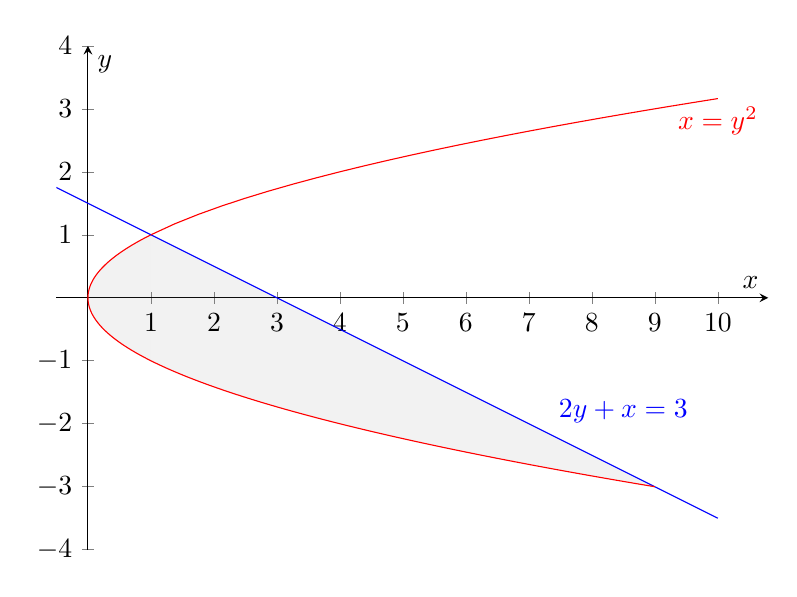
\begin{tikzpicture}
\begin{axis}[
x =0.8 cm, y=0.8 cm,
 axis lines=middle,
  xmin=-0.5,xmax=10.8,ymin=-4,ymax=4,
  xtick distance=1,
  ytick distance=1,
  xlabel=$x$,
  ylabel=$y$]
\addplot [blue,domain=1:9, samples=1000, name path=B] {(3-x)/2};
\addplot [red,domain=0:1, samples=1000, name path=C] {-sqrt(x)};
\addplot [red,domain=1:9, samples=1000, name path=D] {-sqrt(x)};
\addplot [red,domain=0:1, samples=1000, name path=A] {sqrt(x)};
\addplot [red,domain=1:10] {sqrt(x)};
\addplot [blue,domain=-2:1] {(3-x)/2};
\addplot [blue,domain=9:10] {(3-x)/2};
\addplot[gray,opacity=0.1] fill between[of=C and A];
\addplot[gray,opacity=0.1] fill between[of=D and B];
% \draw[dashed,<->] (0.15,0.3873) -- (0.15,1);
% \draw[dashed,<->] (0.7,0.49) -- (0.7,1);
\draw[red] (10,2.8) node{$x=y^2$};
\draw[blue] (8.5,-1.8) node{$2y+x=3$};
% \draw (-2,1) -- (1.2,1) node [right] {$y=1$};
% \draw (0.45,0.2025) -- (0.45,0.6708);
% \draw (0.46,0.67823) -- (0.46,0.2116);
\end{axis}
\end{tikzpicture}
		\end{center}
    \item Gambarkan daerah yang dibatasi oleh kurva-kurva $y=\sqrt{x}, y=2,$ dan $x=0$, kemudian dapatkan volume benda putar jika daerah tersebut diputar pada garis $x=-2$.
    \begin{center} 
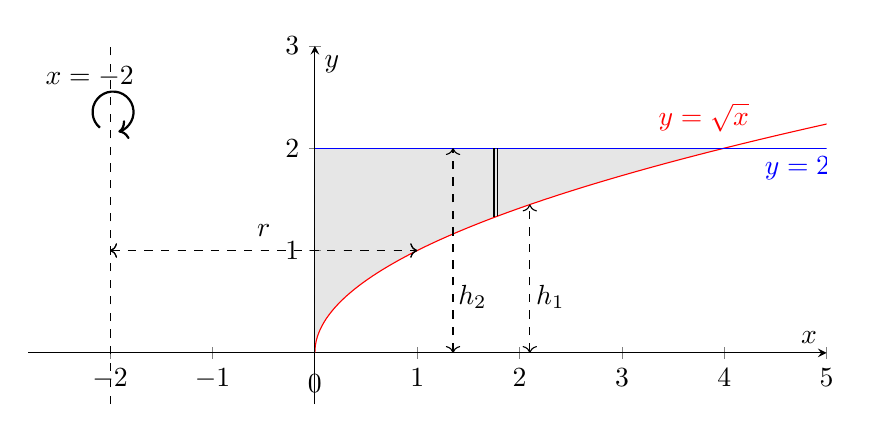
\begin{tikzpicture}
\begin{axis}[
x =1.3 cm, y=1.3 cm,
axis lines=middle,
xmin=-2.8,xmax=5,
ymin=-0.5,ymax=3,
xtick distance=1,
ytick distance=1,
xlabel=$x$,
ylabel=$y$
]

% Kurva y = sqrt(x)
\addplot [red,domain=0:4, samples=1000, name path=A] {sqrt(x)};
\addplot [red,domain=4:5, samples=1000] {sqrt(x)};

% Garis y = 2
\addplot [blue,domain=0:4, samples=1000, name path=B] {2};
\addplot [blue,domain=4:5, samples=1000] {2};

% Daerah arsiran
\addplot[gray,opacity=0.2] fill between[of=A and B, soft clip={domain=0:4}];


% Garis x = 0
\draw[dashed] (0,0) -- (0,2);

% Sumbu putar x = -2
\draw[dashed] (-2,-0.5) -- (-2,3);
\draw (-2.2,2.7) node{$x=-2$};

\draw (1.78, 2) -- (1.78, {sqrt(1.78)});
\draw (1.75, 2) -- (1.75, {sqrt(1.75)});

% Penanda jari-jari
\draw[dashed,<->] (-2,1) -- (1,1);
\draw (-0.5,1.2) node{$r$};
\draw[dashed,<->] (-2,1) -- (1,1);
\draw[dashed,<->]  (1.35,0) -- (1.35,2);
\draw[dashed,<->]  (2.1,0) -- (2.1,{sqrt(2.1)});
\draw (2.3,0.55) node{$h_1$};
\draw (1.54,0.55) node{$h_2$};

% Label kurva
\draw[red] (3.8,2.3) node{$y=\sqrt{x}$};
\draw[blue] (4.3,1.8) node[right] {$y=2$};

% Label x=0
\draw (0,-0.3) node{$0$};
\draw[thick,->]
(-2.1,2.2)
arc[start angle=230,end angle=-75,radius=0.2];



\end{axis}
\end{tikzpicture}
\end{center}
    \item Diberikan persamaan parametrik $x=t^2+1, y=t, 0\leq t\leq 5$.
    \begin{enumerate}
        \item Buatlah sketsa kurva tersebut dengan mengeliminasi parameter $t$
        \item Dapatkan persamaan garis singgung dari persamaan parametrik tersebut saat $t=\frac{1}{2}$.
    \end{enumerate}
    \item Dapatkan luas daerah dari irisan kardioida $r=2-2\cos\theta$ dan kardioida $r=2+2\cos\theta$.
    \item Dapatkan lima suku pertama polinomial Maclaurin untuk fungsi $f(x)=e^{-x^2}$.
\end{enumerate}
\vfill
\begin{center}
    \noindent\rule{0.366416\linewidth}{2pt} \textbf{ Selamat Mengerjakan } \rule{0.366416\linewidth}{2pt}
\end{center}
\begin{center}
    \textit{"Jujur adalah kunci kesuksesan"}
\end{center}

\newpage
\begin{center}
	{\underline{\textbf{\MakeUppercase{EVALUASI AKHIR SEMESTER BERSAMA GENAP 2023/2024}}}}
    \end{center}

    \begin{center}
	\begin{tabular}{lcl}
		Mata kuliah/SKS & : & Kalkulus 2 ( SM234201 ) / 3 SKS\\
		Hari, Tanggal & : & Rabu, 26 Juni 2024\\
		Waktu & : & 09.00-10.40 WIB (100 menit)\\
		Sifat & : & Tertutup\\
		Kelas & : & 15-27, 102\\
  ~
	\end{tabular}

    \noindent\rule{\textwidth}{2.pt}
    \noindent Diberikan 5 soal, dengan bobot nilai masing-masing soal sama dan boleh dikerjakan tidak berurutan.\\
    Tuliskan: Nama, NRP, dan Nomor Kelas pada lembar jawaban Anda.\\
    \textbf{\MakeUppercase{dilarang membawa/menggunakan kalkulator dan alat komunikasi}}\\
    {\textbf{\MakeUppercase{dilarang memberikan/menerima jawaban selama ujian}}}\\
    {\textbf{"Setiap tindak kecurangan akan mendapat sanksi akademik."}}

	
    \noindent\rule{\textwidth}{2.pt}
        \end{center}
\begin{enumerate}
    \item Dapatkan luas daerah yang dibatasi oleh $y=x^2-4x+3$ dan $y=x+3$.
    \begin{center}
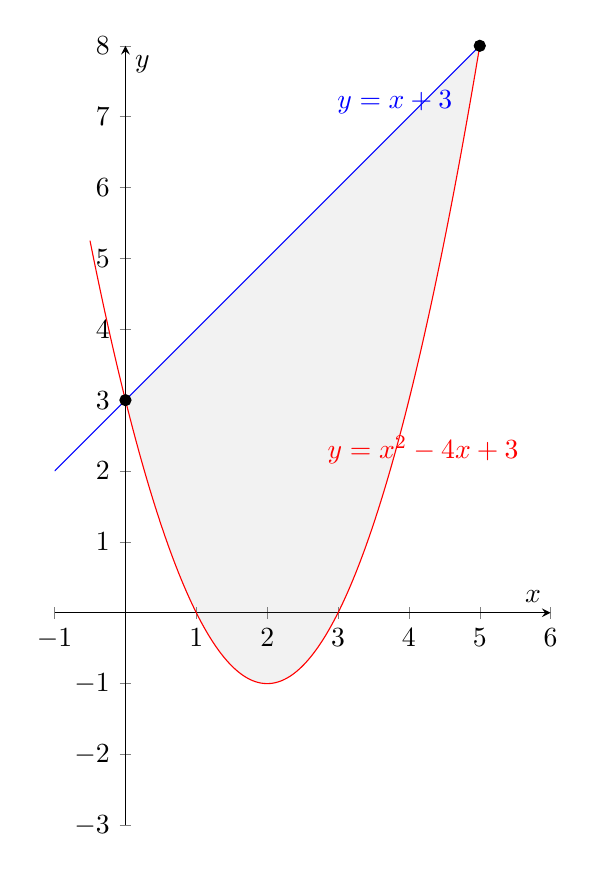
\begin{tikzpicture}
\begin{axis}[
x =0.9 cm, y=0.9 cm,
axis lines=middle,
xmin=-1,xmax=6,
ymin=-3,ymax=8,
xtick distance=1,
ytick distance=1,
xlabel=$x$,
ylabel=$y$
]

% Kurva y = x^2 - 4x + 3
\addplot [red,domain=-0.5:5,samples=1000,name path=A]
{x^2 - 4*x + 3};

% Garis y = x + 3
\addplot [blue,domain=-1:5,samples=1000,name path=B]
{x + 3};

% Arsiran daerah
\addplot[gray,opacity=0.1]
fill between[of=A and B,soft clip={domain=0:5}];

% Label kurva
\draw[red] (4.2,2.3) node{$y=x^2-4x+3$};
\draw[blue] (3.8,7.2) node{$y=x+3$};

% Titik potong
\addplot[
only marks,
mark=*,
mark size=2pt
] coordinates {(0,3) (5,8)};

\end{axis}
\end{tikzpicture}
\end{center}
    \item Dapatkan volume benda putar jika daerah yang dibatasi oleh kurva-kurva $y=\frac{1}{x}, x=2,$ dan $y=2$ diputar terhadap sumbu-$x$. Buatlah sketsa daerah tersebut.
    \begin{center} 
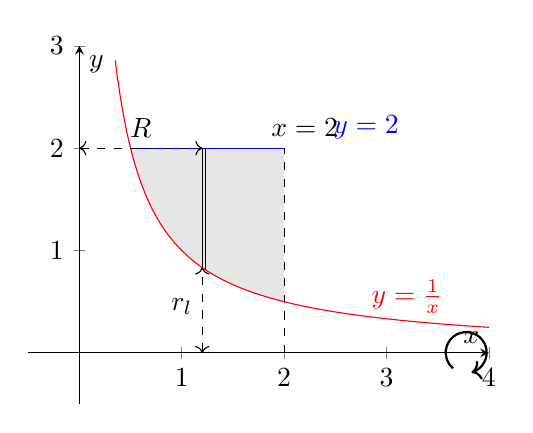
\begin{tikzpicture}
\begin{axis}[
x =1.3 cm, y=1.3 cm,
axis lines=middle,
xmin=-0.5,xmax=4,
ymin=-0.5,ymax=3,
xtick distance=1,
ytick distance=1,
xlabel=$x$,
ylabel=$y$
]

% Kurva y = 1/x
\addplot [red,domain=0.35:2,samples=1000,name path=A] {1/x};
\addplot [red,domain=2:4,samples=1000] {1/x};

% Garis y = 2
\addplot [blue,domain=0.5:2,samples=1000,name path=B] {2};

% Arsiran daerah
\addplot[gray,opacity=0.2]
fill between[of=A and B,soft clip={domain=0.5:2}];

% Garis x = 2
\draw[dashed] (2,0) -- (2,2);

% Contoh washer
\draw (1.2,0.8333) -- (1.2,2);
\draw (1.23,0.813) -- (1.23,2);

% Jari-jari
\draw[dashed,<->] (0,2) -- (1.2,2);
\draw[dashed,<->] (1.2,0) -- (1.2,0.8333);

\draw (0.6,2.2) node{$R$};
\draw (1,0.45) node{$r_l$};

% Label kurva
\draw[red] (3.2,0.55) node{$y=\frac{1}{x}$};
\draw[blue] (2.8,2.2) node{$y=2$};

% Label x = 2
\draw (2.2,2.2) node{$x=2$};

% Simbol rotasi sumbu-x
\draw[thick,->]
(3.65,-0.15)
arc[start angle=230,end angle=-75,radius=0.2];

\end{axis}
\end{tikzpicture}
\end{center}
    \item Diberikan persamaan parametrik $x=\cos 2t, y=3-2\cos 2t, 0\leq t\leq \frac{\pi}{2}$.
    \begin{enumerate}
        \item Dapatkan panjang kurva dari persamaan parametrik
        \item Buatlah sketsa kurva tersebut.
    \end{enumerate}
    \item Dapatkan luas daerah yang berada di dalam $r=2-2\cos\theta$ dan di luar kardioida $r=2+2\cos\theta$.
    \item Dapatkan deret Maclaurin untuk fungsi $f(x)=\ln(1+x)$.
\end{enumerate}
\vfill
\begin{center}
    \noindent\rule{0.366416\linewidth}{2pt} \textbf{ Selamat Mengerjakan } \rule{0.366416\linewidth}{2pt}
\end{center}
\begin{center}
    \textit{"Jujur adalah kunci kesuksesan"}
\end{center}

\newpage
\begin{center}
	{\underline{\textbf{\MakeUppercase{EVALUASI AKHIR SEMESTER BERSAMA GENAP 2023/2024}}}}
    \end{center}

    \begin{center}
	\begin{tabular}{lcl}
		Mata kuliah/SKS & : & Kalkulus 2 ( SM234201 ) / 3 SKS\\
		Hari, Tanggal & : & Rabu, 26 Juni 2024\\
		Waktu & : & 11.00-12.40 WIB (100 menit)\\
		Sifat & : & Tertutup\\
		Kelas & : & 31-38, 104\\
  ~
	\end{tabular}

    \noindent\rule{\textwidth}{2.pt}
    \noindent Diberikan 5 soal, dengan bobot nilai masing-masing soal sama dan boleh dikerjakan tidak berurutan.\\
    Tuliskan: Nama, NRP, dan Nomor Kelas pada lembar jawaban Anda.\\
    \textbf{\MakeUppercase{dilarang membawa/menggunakan kalkulator dan alat komunikasi}}\\
    {\textbf{\MakeUppercase{dilarang memberikan/menerima jawaban selama ujian}}}\\
    {\textbf{"Setiap tindak kecurangan akan mendapat sanksi akademik."}}

	
    \noindent\rule{\textwidth}{2.pt}
        \end{center}
\begin{enumerate}
    \item Dapatkan luas daerah yang dibatasi oleh $y=-x^2+2x+3$ dan $y+2x=3$.
    \begin{center}
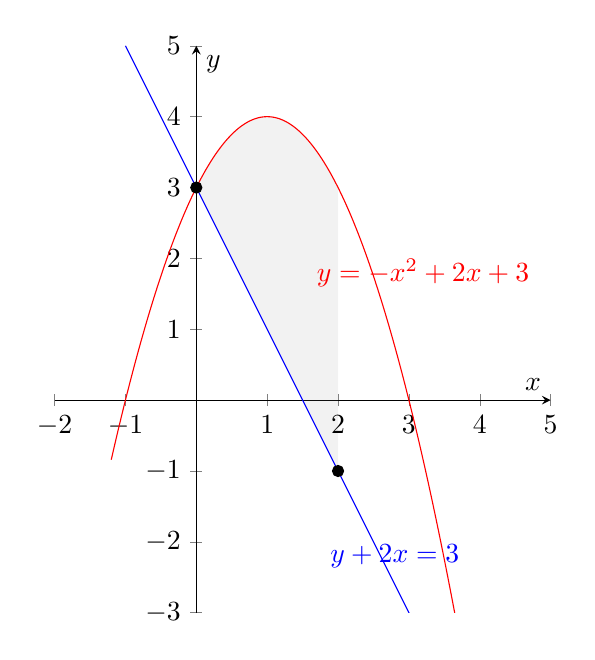
\begin{tikzpicture}
\begin{axis}[
x =0.9 cm, y=0.9 cm,
axis lines=middle,
xmin=-2,xmax=5,
ymin=-3,ymax=5,
xtick distance=1,
ytick distance=1,
xlabel=$x$,
ylabel=$y$
]

% Kurva y = -x^2 + 2x + 3
\addplot [
red,
domain=-1.2:4.2,
samples=1000,
name path=A
]
{-x^2 + 2*x + 3};

% Garis y + 2x = 3  --> y = 3 - 2x
\addplot [
blue,
domain=-1:4,
samples=1000,
name path=B
]
{3 - 2*x};

% Arsiran daerah
\addplot[
gray,
opacity=0.1
]
fill between[
of=A and B,
soft clip={domain=0:2}
];

% Label kurva
\draw[red] (3.2,1.8) node{$y=-x^2+2x+3$};

% Label garis
\draw[blue] (2.8,-2.2) node{$y+2x=3$};

% Titik potong
\addplot[
only marks,
mark=*,
mark size=2pt
]
coordinates {(0,3) (2,-1)};

\end{axis}
\end{tikzpicture}
\end{center}
    \item Gambarkan daerah yang dibatasi oleh kurva-kurva $y=2x-x^2$ dan $y=x^2-2x$. Menggunakan Dalil Guldin I, dapatkan volume benda padat jika daerah tersebut diputar terhadap garis $y=2$.
    \begin{center} 
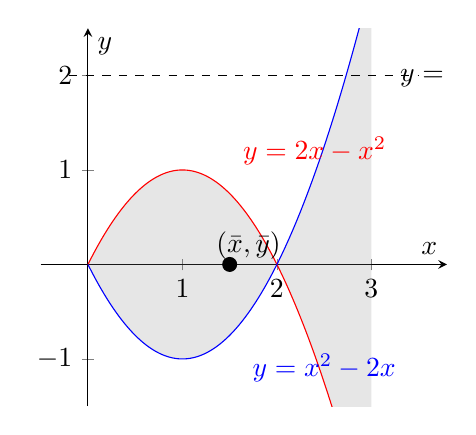
\begin{tikzpicture}
\begin{axis}[
x =1.2 cm, y=1.2 cm,
axis lines=middle,
xmin=-0.5,xmax=3.8,
ymin=-1.5,ymax=2.5,
xtick distance=1,
ytick distance=1,
xlabel=$x$,
ylabel=$y$
]

% Kurva y = 2x - x^2
\addplot [red,domain=0:3,samples=1000,name path=A] {2*x - x^2};
\addplot [red,domain=3:3.5,samples=1000] {2*x - x^2};

% Kurva y = x^2 - 2x
\addplot [blue,domain=0:3,samples=1000,name path=B] {x^2 - 2*x};
\addplot [blue,domain=3:3.5,samples=1000] {x^2 - 2*x};

% Arsiran daerah
\addplot[gray,opacity=0.2]
fill between[of=A and B,soft clip={domain=0:3}];

% Garis y = 2
\draw[dashed] (-0.2,2) -- (3.5,2);
\draw (3.65,2) node{$y=2$};

% Titik berat
\addplot[
only marks,
mark=*,
mark size=2.5pt
] coordinates {(1.5,0)};

\draw (1.7,0.2) node{$(\bar{x},\bar{y})$};

% Label kurva
\draw[red] (2.4,1.2) node{$y=2x-x^2$};
\draw[blue] (2.5,-1.1) node{$y=x^2-2x$};

\end{axis}
\end{tikzpicture}
\end{center}
    \item Diberikan persamaan parametrik $x=\sin t, y=1+2\sin t, 0\leq t\leq \frac{\pi}{2}$.
    \begin{enumerate}
        \item Dapatkan panjang kurva dari persamaan parametrik
        \item Buatlah sketsa kurva tersebut.
    \end{enumerate}
    \item Dapatkan luas daerah yang berada di dalam lingkaran $r=4\sin\theta$ dan di luar lingkaran  $r=4\cos\theta$.
    \item Dapatkan deret Taylor untuk fungsi $f(x)=\dfrac{1}{5-4x}$ di sekitar $x=1$.
\end{enumerate}
\vfill
\begin{center}
    \noindent\rule{0.366416\linewidth}{2pt} \textbf{ Selamat Mengerjakan } \rule{0.366416\linewidth}{2pt}
\end{center}
\begin{center}
    \textit{"Jujur adalah kunci kesuksesan"}
\end{center}

\newpage
\begin{center}
	{\underline{\textbf{\MakeUppercase{EVALUASI AKHIR SEMESTER BERSAMA GENAP 2023/2024}}}}
    \end{center}

    \begin{center}
	\begin{tabular}{lcl}
		Mata kuliah/SKS & : & Kalkulus 2 ( SM234201 ) / 3 SKS\\
		Hari, Tanggal & : & Rabu, 26 Juni 2024\\
		Waktu & : & 13.30-15.10 WIB (100 menit)\\
		Sifat & : & Tertutup\\
		Kelas & : & 40-46, 105\\
  ~
	\end{tabular}

    \noindent\rule{\textwidth}{2.pt}
    \noindent Diberikan 5 soal, dengan bobot nilai masing-masing soal sama dan boleh dikerjakan tidak berurutan.\\
    Tuliskan: Nama, NRP, dan Nomor Kelas pada lembar jawaban Anda.\\
    \textbf{\MakeUppercase{dilarang membawa/menggunakan kalkulator dan alat komunikasi}}\\
    {\textbf{\MakeUppercase{dilarang memberikan/menerima jawaban selama ujian}}}\\
    {\textbf{"Setiap tindak kecurangan akan mendapat sanksi akademik."}}

	
    \noindent\rule{\textwidth}{2.pt}
        \end{center}
\begin{enumerate}
    \item Dapatkan luas daerah yang dibatasi oleh $y=\sqrt{x+2}$; $y=x$ dan $y=0$.
    \begin{center}
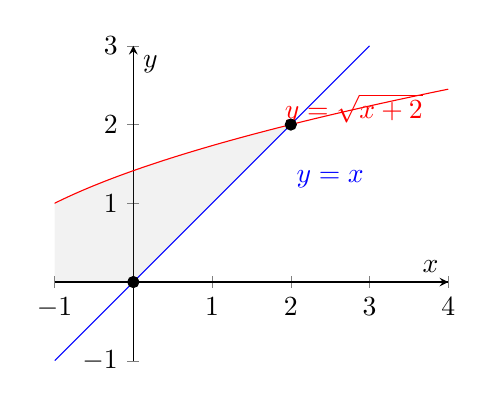
\begin{tikzpicture}
\begin{axis}[
x =1 cm, y=1 cm,
axis lines=middle,
xmin=-1,xmax=4,
ymin=-1,ymax=3,
xtick distance=1,
ytick distance=1,
xlabel=$x$,
ylabel=$y$
]

% Kurva y = sqrt(x+2)
\addplot [red,domain=-2:4,samples=1000,name path=A]
{sqrt(x+2)};

% Garis y = x
\addplot [blue,domain=-1:3,samples=1000,name path=B]
{x};

% Sumbu-x
\addplot [black,domain=-1:4,name path=C]
{0};

% Arsiran daerah antara y=sqrt(x+2) dan y=0
\addplot[gray,opacity=0.1]
fill between[of=A and C,soft clip={domain=-2:0}];

% Arsiran daerah antara y=sqrt(x+2) dan y=x
\addplot[gray,opacity=0.1]
fill between[of=A and B,soft clip={domain=0:2}];

% Label kurva
\draw[red] (2.8,2.2) node{$y=\sqrt{x+2}$};
\draw[blue] (2.5,1.3) node{$y=x$};

% Titik potong
\addplot[
only marks,
mark=*,
mark size=2pt
] coordinates {(-2,0) (0,0) (2,2)};

\end{axis}
\end{tikzpicture}
\end{center}
    \item Dapatkan luas daerah yang dibatasi oleh kurva $y=-x^2+x$ dan sumbu-$x$. Menggunakan Dalil Guldin I, dapatkan volume benda padat jika daerah tersebut diputar pada garis $x=4$.
\begin{center} 
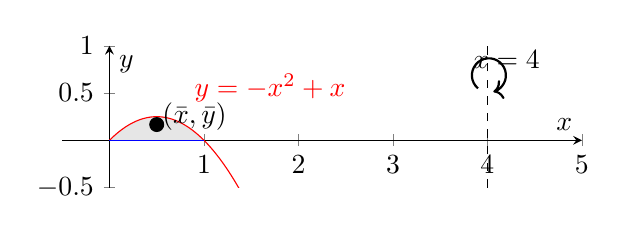
\begin{tikzpicture}
\begin{axis}[
x =1.2 cm, y=1.2 cm,
axis lines=middle,
xmin=-0.5,xmax=5,
ymin=-0.5,ymax=1,
xtick distance=1,
ytick distance=0.5,
xlabel=$x$,
ylabel=$y$
]

% Kurva y = -x^2 + x
\addplot [red,domain=0:1,samples=1000,name path=A] {-x^2 + x};
\addplot [red,domain=1:2,samples=1000] {-x^2 + x};

% Sumbu-x
\addplot [blue,domain=0:1,name path=B] {0};

% Arsiran daerah
\addplot[gray,opacity=0.2]
fill between[of=A and B,soft clip={domain=0:1}];

% Garis sumbu putar x = 4
\draw[dashed] (4,-0.5) -- (4,1);
\draw (4.2,0.85) node{$x=4$};

% Titik berat
\addplot[
only marks,
mark=*,
mark size=2.5pt
] coordinates {(0.5,0.1667)};

\draw (0.9,0.25) node{$(\bar{x},\bar{y})$};

% Label kurva
\draw[red] (1.7,0.55) node{$y=-x^2+x$};

% Simbol rotasi
\draw[thick,->]
(3.9,0.55)
arc[start angle=230,end angle=-75,radius=0.18];

\end{axis}
\end{tikzpicture}
\end{center}
    \item Dapatkan persamaan garis singgung kurva $x=t+\cos t$, $y=2+\sin t$ saat $t=0$
    \item Dapatkan luas daerah dari irisan lingkaran $r=4\sin\theta$ dan lingkaran $r=4\cos\theta$.
    \item Dapatkan deret Maclaurin untuk fungsi $f(x)=xe^x$.
\end{enumerate}
\vfill
\begin{center}
    \noindent\rule{0.366416\linewidth}{2pt} \textbf{ Selamat Mengerjakan } \rule{0.366416\linewidth}{2pt}
\end{center}
\begin{center}
    \textit{"Jujur adalah kunci kesuksesan"}
\end{center}

\newpage
\begin{center}
	{\underline
{\textbf{\MakeUppercase{EVALUASI AKHIR SEMESTER BERSAMA GENAP 2023/2024}}}}
    \end{center}

    \begin{center}
	\begin{tabular}{lcl}
		Mata kuliah/SKS & : & Kalkulus 2 ( SM234201 ) / 3 SKS\\
		Hari, Tanggal & : & Kamis, 27 Juni 2024\\
		Waktu & : & 11.00-12.40 WIB (100 menit)\\
		Sifat & : & Tertutup\\
		Kelas & : & 48-60, 107\\
  ~
	\end{tabular}

    \noindent\rule{\textwidth}{2.pt}
    \noindent Diberikan 5 soal, dengan bobot nilai masing-masing soal sama dan boleh dikerjakan tidak berurutan.\\
    Tuliskan: Nama, NRP, dan Nomor Kelas pada lembar jawaban Anda.\\
    \textbf{\MakeUppercase{dilarang membawa/menggunakan kalkulator dan alat komunikasi}}\\
    {\textbf{\MakeUppercase{dilarang memberikan/menerima jawaban selama ujian}}}\\
    {\textbf{"Setiap tindak kecurangan akan mendapat sanksi akademik."}}

	
    \noindent\rule{\textwidth}{2.pt}
        \end{center}
\begin{enumerate}
    \item Dapatkan luas daerah yang dibatasi oleh $x=y^3-y$ dan $x=0$.
% \begin{center}
% \begin{tikzpicture}
% \begin{axis}[
% x =1 cm, y=1 cm,
% axis lines=middle,
% xmin=-3,xmax=3,
% ymin=-2,ymax=2,
% xtick distance=1,
% ytick distance=1,
% xlabel=$x$,
% ylabel=$y$
% ]

% % Kurva x = y^3 - y
% \addplot [
% red,
% domain=-1.5:1.5,
% samples=1000,
% variable=\y
% ]
% ({\y^3-\y},{\y});

% % Garis x = 0
% \addplot [
% blue,
% domain=-1.2:1.2,
% samples=1000
% ]
% ({0},{x});

% % Arsiran daerah
% \addplot [
% gray,
% opacity=0.15
% ]
% fill between[
% of={
% \addplot [
% domain=-1:1,
% samples=500,
% variable=\y
% ]
% ({\y^3-\y},{\y});
% }
% and {
% \addplot [
% domain=-1:1,
% samples=500,
% variable=\y
% ]
% ({0},{\y});
% }
% ];

% % Label kurva
% \draw[red] (2.1,1.3) node{$x=y^3-y$};

% % Label garis
% \draw[blue] (0.45,1.5) node{$x=0$};

% % Titik potong
% \addplot[
% only marks,
% mark=*,
% mark size=2pt
% ]
% coordinates {(0,-1) (0,0) (0,1)};

% \end{axis}
% \end{tikzpicture}
% \end{center}
    \item Gambarkan daerah di kuadran I yang dibatasi oleh kurva-kurva $y=x^2$, $y=8-2x$ dan sumbu-$y$. Dapatkan volume benda putar jika daerah tersebut diputar pada sumbu-$x$.
%     \begin{center} 
% \begin{tikzpicture}
% \begin{axis}[
% x =0.9 cm, y=0.9 cm,
% axis lines=middle,
% xmin=-0.5,xmax=5,
% ymin=-0.5,ymax=9,
% xtick distance=1,
% ytick distance=1,
% xlabel=$x$,
% ylabel=$y$
% ]

% % Kurva y = x^2
% \addplot [red,domain=0:2,samples=1000,name path=A] {x^2};
% \addplot [red,domain=2:3,samples=1000] {x^2};

% % Garis y = 8 - 2x
% \addplot [blue,domain=0:4,samples=1000,name path=B] {8 - 2*x};

% % Arsiran daerah
% \addplot[gray,opacity=0.2]
% fill between[of=A and B,soft clip={domain=0:2}];

% % Garis sumbu-y
% \draw[dashed] (0,0) -- (0,8);

% % Contoh shell
% \draw (1.35,{1.35^2}) -- (1.35,{8-2*1.35});
% \draw (1.38,{1.38^2}) -- (1.38,{8-2*1.38});

% % Penanda jari-jari
% \draw[dashed,<->] (0,1.5) -- (1.35,1.5);
% \draw (0.7,1.8) node{$r$};

% % Penanda tinggi
% \draw[dashed,<->] (2.2,{2.2^2}) -- (2.2,{8-2*2.2});
% \draw (2.45,3.8) node{$h$};

% % Label kurva
% \draw[red] (2.5,6.8) node{$y=x^2$};
% \draw[blue] (3.2,1.8) node{$y=8-2x$};

% % Simbol rotasi sumbu-x
% \draw[thick,->]
% (0.45,-0.18)
% arc[start angle=230,end angle=-75,radius=0.2];

% \end{axis}
% \end{tikzpicture}
% \end{center}
    \item Hitung panjang busur kurva $x=a(t-\sin t)$, $y=a(1-\cos t)$ pada $0\leq t\leq 2\pi$.
    \item Hitung luas daerah yang diperoleh dari irisan kurva $r=3\cos \theta$ dan $r=1+\cos\theta$.
    \item Dapatkan polinomial Taylor untuk fungsi $f(x)=x\cos x$ di sekitar $x=\pi$ hingga suku ke empat.
\end{enumerate}
\vfill
\begin{center}
    \noindent\rule{0.366416\linewidth}{2pt} \textbf{ Selamat Mengerjakan } \rule{0.366416\linewidth}{2pt}
\end{center}
\begin{center}
    \textit{"Jujur adalah kunci kesuksesan"}
\end{center}

\end{document}
